%% ---------------------------------------------------------------------------
\documentclass[openany, twoside, a5paper, 10pt]{book}
%% ---------------------------------------------------------------------------
\usepackage[cp1251]{inputenc}
\usepackage[english,russian]{babel}
%% ---------------------------------------------------------------------------
\usepackage{indentfirst}
\frenchspacing
%% ---------------------------------------------------------------------------
\usepackage{url}
%% ---------------------------------------------------------------------------
\usepackage[dvips]{graphicx}
%\usepackage[pdftex]{graphicx}
%\usepackage{epstopdf}
%% ---------------------------------------------------------------------------
\usepackage{amsmath}
\usepackage{amssymb}
\usepackage{amscd}
\usepackage{bm}
\usepackage{ifmtarg}
%% ---------------------------------------------------------------------------
%\usepackage{soul}
%% ---------------------------------------------------------------------------
%\sloppy
%% ---------------------------------------------------------------------------
% a5paper: 148 x 210
% print area: 110 x 180
% top = bottom = (210 - 180) / 2 = 15
% left = right = (148 - 110) / 2 = 19
\usepackage[%
    left=1.9cm,%
    top=1.5cm,%
    right=1.9cm,%
    bottom=1.5cm,%
    headsep=0.2cm,%
    footskip=0.5cm,%
    includehead,%
    includefoot]{geometry}
%% ---------------------------------------------------------------------------
%% set lengthes
\newlength{\maxpicturewidth}
\setlength{\maxpicturewidth}{\textwidth }
\newlength{\maxpictureheight}
\setlength{\maxpictureheight}{\textheight }
%% ---------------------------------------------------------------------------
\usepackage{titlesec,titletoc}
%% ---------------------------------------------------------------------------
\setcounter{secnumdepth}{-1}
%% ---------------------------------------------------------------------------
\titleformat{\chapter}[display]
{\normalfont\huge\filcenter\bfseries}{}{20pt}{\Huge}
%% ---------------------------------------------------------------------------
\makeatletter
%% ---------------------------------------------------------------------------
% \Title[thanksto]{title}{name}{university}{city}{country}
\def\Title{%
    \@ifnextchar[{\TitleFootnote}{\TitleNoFootnote}
}
\newcounter{aster}
\setcounter{aster}{1}
%\renewcommand{\thefootnote}{\fnsymbol{footnote}}
\renewcommand{\thefootnote}{\fnsymbol{aster}}

\def\TitleFootnote[#1]#2#3#4#5#6{%
    \par
    \begin{centering}
        \medskip
        {\Large
         \textbf{#2}\@ifmtarg{#1}{}{\footnote{#1}}}\\
        \medskip
            #3\\
            \textit{#4, #5, #6}\\
        \smallskip
    \end{centering}
    \@afterheading
}
\def\TitleNoFootnote#1#2#3#4#5{%
    \par
    \begin{centering}
        \medskip
        {\Large
         \textbf{#1}}\\
        \medskip
            #2\\
            \textit{#3, #4, #5}\\
        \smallskip
    \end{centering}
    \@afterheading
}
%% ---------------------------------------------------------------------------
\newenvironment{references_rus}{%
    \par
    \medskip
    \centerline{\textbf{������ ����������}}
    \nopagebreak
    \medskip
    \@afterheading
    \begin{enumerate}
     \parsep=0pt plus 1pt
     \parskip=\parsep
     \itemsep=\parsep
}
{\end{enumerate}}
\newenvironment{references_eng}{%
    \par
    \medskip
    \centerline{\textbf{References}}
    \nopagebreak
    \medskip
    \@afterheading
    \begin{enumerate}
     \parsep=0pt plus 1pt
     \parskip=\parsep
     \itemsep=\parsep
}
{\end{enumerate}}
%% ---------------------------------------------------------------------------
\makeatother
%% ---------------------------------------------------------------------------

\begin{document}

%% ---------------------------------------------------------------------------
\renewcommand{\indexname}{Author index}
%% ---------------------------------------------------------------------------
%%%%%%%%%%%%%%%%% your_thesis_eng.tex %%%%%%%%%%%%%%%%%
%
% This is the template file for ORM 2018 proceedings.
%
% Please, fill in following the directions below.
%
%%%%%%%%%%%%%%%%%%%%%%%%%%%%%%%%%%%%%%%%%%%%%%%%%%%%%%%

\Title
{%
% Insert your title here
Asymptotic properties of tandem service and control operation in a class of cyclic algorithms with prolongation
}
{%
% Insert the authors' names here
V.M.~Kocheganov, A.V.~Zorine%
}
{%
% Insert your institution here
N.I. Lobachevsky National Research State University of Nizhny Novgorod%
}
{%
% Insert your city here
Nizhny Novgorod
}
{%
% Insert your country here
Russia
}

% Insert your thesis here.
% The entire submission should not exceed 5 pages if you plan a publication in conference proceedings.
%
% ATTENTION: Using 'thebibliography' environment is not allowed.
% Use 'references_eng' environment below to format the list of references.
% Please note that the latter environment does not provide automatic
% citation facilities. Cite manually using square brackets,
% e.g., [1], [2, 3], [4--6].
%


Operations research is a field of mathematics which deals with finding optimal way of \textit{operation} on different objects. The nature of these operations might contain very complex stochastic grain.  Once the objects are customers or demands and the operation is service and control, queuing theory methods can be used. Queuing theory approaches can be divided in two groups. The first group of methods is classical and assume homogeneity of all customers as well as that of all operations on the customers. For the first time such constraints were considered in the early XX century by F.~Johanssen, A.K.~Erlang, A.Ya.~Khinchine, F.~Pollaczek, C.~Palm,
D. Kendall. During the second half of the XX century this sort of customers and operations on them have been investigated by A.N.~Kolmogorov, B.V.~Gnedenko, T.D.~Saati, Yu.V.~Prokhorov, E.S.~Ventsel et~al. 

Though there are a lot of cases where homogeneity assumptions do not hold: information flows processing in local-area computer networks and telecommunication networks, control of conflicting flows of aircrafts at passage of intersecting air lanes, conflicting transport flows control at intersections with complicated crossing geometry etc.
The second group of queuing theory methods deal with nonhomogeneous customers and nonhomogeneous operations on these customers. This is done via solving following fundamental problems: 1) classification of nonhomogeneous customers
and description of flows of nonhomogeneous customers; 2) formation and development of control algorithms of conflicting flows of nonhomogeneous customers. In this paper we describe one of the problems that can be solved with second group of queuing theory methods.


% Insert your figure, if needed.
\begin{figure}[h]
  \centering
  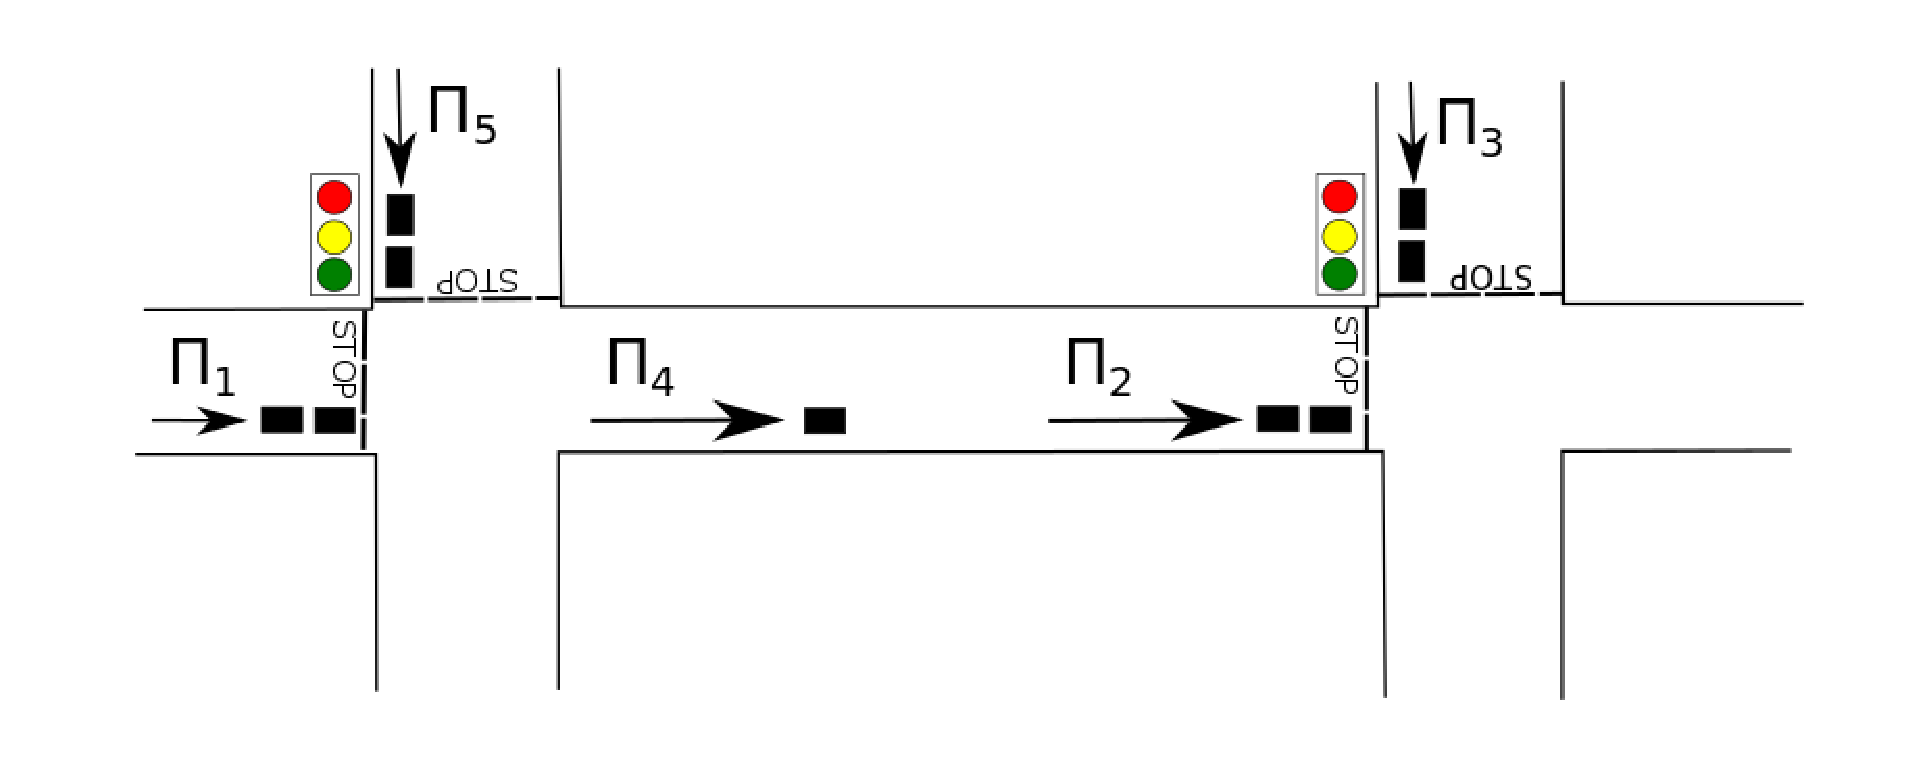
\includegraphics[width=1\maxpicturewidth]{Crossroads.eps}
  \center{Fig.~1. Tandem of crossroads}
     \label{crossroads}
\end{figure}


Consider a real-life system of tandem of two consecutive crossroads
(Fig.~1).
The input flows are flows of vehicles. The flows $\Pi_1$ and $\Pi_5$ at the first crossroad are
conflicting; $\Pi_2$ and $\Pi_3$ at the second crossroad are also conflicting. Every vehicle from
the flow $\Pi_1$ after passing the first road intersection joints the flow $\Pi_4$ and enters the queue
$O_4$. After some random time interval the vehicle arrives to the next road intersection. Such a pair of crossroads is an instance of a more general queuing model described below. 

Consider a queuing system with  four input flows of customers $\Pi_1$, $\Pi_2$, $\Pi_3$, and $\Pi_4$ entering the single server queueing
system ($\Pi_5$ flow has no effect on system behaviour and is omitted in remaining discussion). Customers in the input flow $\Pi_j$, $j \in \{1,2,3,4\}$ join a queue $O_j$ with an
unlimited capacity. For $j \in \{1,2,3\}$ the discipline of the queue $O_j$ is FIFO (First In First
Out). Discipline of the queue $O_4$ will be described later. The input flows $\Pi_1$ and $\Pi_3$ are
generated by an external environment, which has only one state. Each of these flows is a nonordinary
Poisson flow. Denote by $\lambda_1$ and $\lambda_3$ the intensities of bulk arrivals for the flows
$\Pi_1$ and $\Pi_3$ respectively. The probability generating function of number of customers in a
bulk in the flow $\Pi_j$ is $f_j(z) = \sum_{\nu=1}^{\infty} p_{\nu}^{(j)} z ^{\nu}, \quad j\in \{1,3\}$.
We assume that $f_j(z)$ converges for any $z\in \mathbb{C}$ such that $|z|<(1+\varepsilon)$,
$\varepsilon>0$. Here $p_{\nu}^{(j)}$ is the probability of a bulk size in flow $\Pi_j$ being
exactly $\nu=1$, $2$, \ldots. Having been serviced the customers from $O_1$ come back to the system
as the $\Pi_4$ customers. The $\Pi_4$ customers in turn after service enter the system as the
$\Pi_2$ ones. The flows $\Pi_2$ and $\Pi_3$ are conflicting in the sense that their customers can't
be serviced simultaneously. This implies that the problem can't be reduced to a problem with fewer
input flows by merging the flows together.


In order to describe the server behavior positive integers $d$, $n_0$, $n_1$, $\ldots$,
$n_d$ are fixed and a finite set $\Gamma=\{\Gamma^{(k,r)} \colon k=0,1,\ldots,d; r=1,2,\ldots
n_k\}$ of states server can reside in is introduced. At the state $\Gamma^{(k,r)}$ the server stays during a constant 
time $T^{(k,r)}$. We will assume, that for each fixed $k^*$ cycle subset $\{\Gamma^{(k^*,r)} \colon r=1,2,\ldots
n_k^*\} = C_{k^*}^{\mathrm{N}} \cup  C_{k^*}^{\mathrm{O}} \cup  C_{k^*}^{\mathrm{I}}$, that is consists of three disjoint sets called neutral, output and input sets of states.  In more details server is described in~[1].

In general, service durations of different customers can be dependent and may have different laws of
probability distributions. So, saturation flows will be used to define the service process. The
saturation flow $\Pi^{\mathrm{\text{sat}}}_j$, $j \in \{1,2,3,4\}$, is defined as a virtual output
flow under the maximum usage of the server and unlimited number of customer in the queue $O_j$. The
saturation flow $\Pi^{\mathrm{\text{sat}}}_j$, $j\in \{1,2,3\}$ contains a non-random number
$\ell({k,r,j)}\geqslant0$ of customers in the server state $\Gamma^{(k,r)}$.





The queuing system under investigation can be regarded as a cybernetic control system, it helps to
rigorously construct a formal stochastic model~[2]. There are following blocks present in the system: 1)~the external
environment with one state; 2) input poles of the first type~--- the input flows $\Pi_1$, $\Pi_2$,
$\Pi_3$, and $\Pi_4$; 3) input poles of the second type~--- the saturation flows
$\Pi^{\mathrm{\text{sat}}}_1$, $\Pi^{\mathrm{\text{sat}}}_2$, $\Pi^{\mathrm{\text{sat}}}_3$, and
$\Pi^{\mathrm{\text{sat}}}_4$; 4)~an external memory~--- the queues $O_1$, $O_2$, $O_3$, and $O_4$;
5)~an information processing device for the external memory~--- the queue discipline units
$\delta_1$, $\delta_2$, $\delta_3$, and $\delta_4$; 6) an internal memory --- the server (OY); 7)~an
information processing device for internal memory~--- the graph of server state transitions;
8)~output poles~--- the output flows $\Pi^{\mathrm{\text{out}}}_1$, $\Pi^{\mathrm{\text{out}}}_2$,
$\Pi^{\mathrm{\text{out}}}_3$, and $\Pi^{\mathrm{\text{out}}}_4$. 

Let us  introduce the following variables and elements along with their
value ranges. To fix a discrete time scale consider the epochs $\tau_0=0$, $\tau_1$, $\tau_2$,
$\ldots$ when the server changes its state. Let $\Gamma_i\in\Gamma$ be the server state
during the interval $(\tau_{i-1};\tau_i]$, $\varkappa_{j,i} \in \mathbb{Z}_+ $ be the number of customers in
the queue $O_j$ at the instant $\tau_i$, $\eta_{j,i} \in \mathbb{Z}_+$ be the number of customers
arrived into the queue $O_j$ from the flow $\Pi_j$ during the interval $(\tau_{i};\tau_{i+1}]$, $\xi_{j,i} \in
\mathbb{Z}_+$ be the number of customers in the saturation flow $\Pi^{\mathrm{\text{sat}}}_j$ during
the interval $(\tau_{i};\tau_{i+1}]$, $\overline{\xi}_{j,i}\in \mathbb{Z}_+$ be the actual number of 
serviced customers from the queue  $O_j$ during the interval $(\tau_{i};\tau_{i+1}]$, $j\in
\{1,2,3,4\}$.
The server changes its state according to the following rule:
%\begin{equation}
$
\Gamma_{i+1}=h(\Gamma_i,\varkappa_{3,i})
$
%\label{gammaFunc}
%\end{equation}
where the mapping $h(\cdot,\cdot)$ is defined in paper~[1].
Lets define function $\psi(\cdot,\cdot,\cdot)$: $\psi(k;y,u)=C_y^k u^k (1-u)^{y-k}$.
$\psi(k;y,u)$ is probability of arrival of $k$ $\Pi_2$-customers given $O_4$ has $y$ customers and server is in state $\Gamma^{(k,r)}$, that is $u=p_{k,r}$. If $ 0\leqslant k \leqslant y$ does no hold we put $\psi(k;y,u)$ equal $0$.
Mathematical model in more details can be found in work~[3].


We now present several results regarding asymptotic behaviour of described system.
Consider stochastic sequences:
\begin{align}
\label{eq:theMC:1}
&\{(\Gamma_i(\omega), \varkappa_{3,i}(\omega)); i =0, 1, \ldots\},\\
\label{eq:theMC:2}
&\{(\Gamma_i(\omega), \varkappa_{1,i}(\omega),\varkappa_{3,i}(\omega)); i =0, 1, \ldots\},\\
\label{eq:theMC:3}
&\{(\Gamma_i(\omega), \varkappa_{1,i}(\omega),\varkappa_{3,i}(\omega),\varkappa_{4,i}(\omega)); i =0, 1, \ldots\},
\end{align}
which include number of customers $\varkappa_{1, i}(\omega)$, $\varkappa_{3, i}(\omega)$ and $\varkappa_{4, i}(\omega)$ in the queues $O_1$, $O_3$ and $O_4$ respectfully.

\textit{\textbf{Theorem~1.}} 
Let $\Gamma_0=\Gamma^{(k,r)}\in \Gamma$ and $\varkappa_{3,0}=x_{3,0}\in \mathbb{Z}_+$ be fixed. Then the sequence~\eqref{eq:theMC:1} is Markov chain.

\textit{\textbf{Theorem~2.}} 
Let $\Gamma_0=\Gamma^{(k,r)}\in \Gamma$ and $(\varkappa_{1,0}, \varkappa_{3,0})=(x_{1,0}, x_{3,0})\in \mathbb{Z}_+^2$ be fixed. Then the sequence~\eqref{eq:theMC:2} is Markov chain.


\textit{\textbf{Theorem~3.}} 
For Markov chain~\eqref{eq:theMC:1} to have a stationary distribution it is sufficient to satisfy the following inequalitiy
\begin{equation*}
\min_{k=\overline{1,d}} { \frac{\sum_{r = 1}^{n_k} \ell(k,r,3) }{\lambda_3 f_3'(1) \sum_{r=1}^{n_k} T^{(k,r)} }}>1.
\label{sufficient:double}
\end{equation*}


\textit{\textbf{Theorem~4.}} 
For Markov chain~\eqref{eq:theMC:2} to have a stationary distribution it is sufficient to satisfy the following inequalities
\begin{equation*}
\min_{k=\overline{0,d}} { \frac{\sum_{r = 1}^{n_k} \ell(k,r,1) }{\lambda_1 f_1'(1) \sum_{r=1}^{n_k} T^{(k,r)} }}>1, \quad 
\min_{k=\overline{1,d}} { \frac{\sum_{r = 1}^{n_k} \ell(k,r,3) }{\lambda_3 f_3'(1) \sum_{r=1}^{n_k} T^{(k,r)} }}>1.
\label{sufficient:double}
\end{equation*}


\textit{Theorem~1} and \textit{Theorem~3} concern low-priority queue which is also described in~[1,3,4]. \textit{Theorem~2} and \textit{Theorem~4} concern primary input flow queues which are referenced in~[5].

\textit{\textbf{Theorem~5.}} 
For queue sizes in stochastic sequence~\eqref{eq:theMC:3} to be bounded it is sufficient to satisfy assumptions of \textit{Theorem~4} and following inequality:
\begin{equation*}
   % \min_{\substack{k=\overline{1,d}\\ j=1,3}} {\{p_{k,r}\}} > 0.
    \min_{k=\overline{0,d}, r=\overline{1,n_k}} {\{p_{k,r}\}} > 0.
\end{equation*}

\textit{{Proof}} 
Let $(\gamma, x_3) \in \Gamma \times {\mathbb Z}_+$ and  $\Gamma^{(\tilde{k},\tilde{r})}=h(\gamma,x_3)$. Put 
$A_i(w_1,w_3,w_4,\gamma) = \{\omega \colon \varkappa_{1,i}=w_1,\varkappa_{3,i}=w_3, \varkappa_{4,i}=w_4, \Gamma_i=\gamma \}$. Considering recurrent expression for $\varkappa_{4,i+1}$ one has:
\begin{multline*}
    E[\varkappa_{4,i+1} | \varkappa_{1,i}=w_1,\varkappa_{3,i}=w_3, \varkappa_{4,i}=w_4, \Gamma_i=\gamma] = \\
    =
    E[w_4 - \eta_{2,i} +  \min{\{\xi_{1,i}, w_1 + \eta_{1,i} \}} | A_i(w_1,w_3,w_4,\gamma)] \leqslant \\
    \leqslant
     E[w_4 - \eta_{2,i} +  \xi_{1,i} | A_i(w_1,w_3,w_4,\gamma)] =\\ 
     = 
     E[w_4 - \eta_{2,i} +  \ell(\tilde{k},\tilde{r},1) | A_i(w_1,w_3,w_4,\gamma)] = \\ 
    =
   w_4 + \ell(\tilde{k},\tilde{r},1)  -  E[\eta_{2,i} |A_i(w_1,w_3,w_4,\gamma)].
\end{multline*}
From definition of $\psi(\cdot;\cdot,\cdot)$ we get:
\begin{multline*}
  E[\eta_{2,i} | A_i(w_1,w_3,w_4,\gamma)]
=\\ =
\sum_{a=0}^{w_4}  a \psi(a;w_4, p_{\tilde{k},\tilde{r}}) = 
\sum_{a=0}^{w_4} a {{w_4}\choose{a}} p_{\tilde{k},\tilde{r}}^a (1-p_{\tilde{k},\tilde{r}})^{w_4-a} = w_4 p_{\tilde{k},\tilde{r}}.
\end{multline*}
Hence it is true that
   $  E[\varkappa_{4,i+1} | A_i(w_1,w_3,w_4,\gamma)] \leqslant
     w_4 (1-p_{\tilde{k},\tilde{r}}) + \ell(\tilde{k},\tilde{r},1)$.
Using law of total expectation one can get:
\begin{multline*}
    E[\varkappa_{4,i+1}]
    =\sum_{w_1=0}^{\infty} \sum_{w_3=0}^{\infty}  \sum_{w_4=0}^{\infty} \sum_{\gamma \in \Gamma}  E[\varkappa_{4,i+1} | A_i(w_1,w_3,w_4,\gamma)]  \times \\ 
    \times
    {\mathbf P}( A_i(w_1,w_3,w_4,\gamma))  
    \leqslant
    \sum_{w_3=0}^{\infty}  \sum_{w_4=0}^{\infty} \sum_{\gamma \in \Gamma} 
    ( w_4 (1-p_{\tilde{k},\tilde{r}}) + \ell(\tilde{k},\tilde{r},1) ) \times \\   \times 
    {\mathbf P}( A_i(w_1,w_3,w_4,\gamma)) 
    \leqslant
     (1-\min{\{p_{\tilde{k},\tilde{r}}\}}) \times \\ \times \sum_{w_4=0}^{\infty}   w_4 {\mathbf P}(\varkappa_{4,i}=w_4) + \max{\{\ell(\tilde{k},\tilde{r},1)\}} )   \sum_{w_4=0}^{\infty}{\mathbf P}(\varkappa_{4,i}=w_4) = \\
     =
      (1-\min{\{p_{\tilde{k},\tilde{r}}\}})  E[\varkappa_{4,i}] + \max{\{\ell(\tilde{k},\tilde{r},1)\}} ).
\end{multline*}

The sequence $M_0=E[\varkappa_{4,0}]$, $M_{i+1}= (1-\min{\{p_{\tilde{k},\tilde{r}}\}})  M_{i} + \max{\{\ell(\tilde{k},\tilde{r},1)\}} ) $ bounds from above sequence $E[\varkappa_{4,i+1}]$ and under theorem assumptions is limited. It implies $O_4$ queue size $\varkappa_{4,i}$ to be limited. Since conditions of the \textit{Theorem}~4 are satisfied then Markov chain~\eqref{eq:theMC:2} has stationary distribution and queue sizes $\varkappa_{1,i}$ and $\varkappa_{3,i}$ are limited as well. We are done.

\begin{references_eng}
% Insert your list of references here. The order of items in the list must
% agree with the order of their appearance in the text of your thesis.
% Use the '\url' command for citing url-s: e.g., \url{http://http://www.mathopt.org/}.

\item
Kocheganov~V.M., Zorine~A.V. Low-Priority Queue and Server's Steady-State Existence in a Tandem Under Prolongable Cyclic Service // DCCN. Ser. Communications in Computer and Information Science. Springer, Cham. 2016. V.~678. P.~210--221.
\item
  Zorin A.V. Stability of a tandem of queueing systems with Bernoulli noninstantaneous transfer of
  customers~// Theory of Probability and Mathematical Statistics. 2012. V.~84. P.~173--188.
\item
Kocheganov~V.M., Zorine~A.V. Low-Priority Queue Fluctuations in Tandem of Queuing Systems Under Cyclic Control with Prolongations // DCCN. Ser. Communications in Computer and Information Science. 2016. V.~601. P.~268--279.
\item 
Kocheganov~V.M., Zorine~A.V. Sufficient condition of low-priority queue stationary distribution existence in a tandem of queuing systems // Bulletin of the Volga State Academy of Water Transport, 2017, vol.~50, pp.~47--55. (In Russian)
\item
Kocheganov V., Zorine A. Primary input flows in a tandem under prolongable cyclic service // DCCN. 2017. Pp.~517--525.



%   \item % Reference No. 1
%   Taylor~T.T. Article in a collection // Collection title. New York: Springer, 2012. P.~1--21.

%   \item % Reference No. 2
%   Smith~S.S. Book. New York: Springer, 2012.

%   \item
%   Baker~B.B. Journal article // Journal title. 2012. V.~1, \No ~1. P.~1--21.

% ...

\end{references_eng}

%%%%%%%%%%%%%%%%%%%%%%%%%%%%%%%%%%%%%%%%%%%%%%%%%%%%%%%

%\newpage
%\input{your_thesis_rus}
%% ---------------------------------------------------------------------------

\end{document}

%% ---------------------------------------------------------------------------

